\documentclass{article}

\usepackage[utf8]{inputenc}
\usepackage{blindtext}
\usepackage{graphicx}
\usepackage{titling}

\begin{document}

\title{Travail pratique \#1 - IFT-2245} 

\author{Jérémy Coulombe (p1144927) \\ MAUDE SABOURIN (P1141140)}
%\textsrc{\LARGE DÉPARTEMENT D’INFORMATIQUE ET DE RECHERCHE OPÉRATIONNELLE \\
%FACULTÉ DES ARTS ET DES SCIENCES
 %}
%\textsrc{\LARGE TRAVAIL PRÉSENTÉ À LIAM PAULL \\
%\\DANS LE CADRE DU COURS \\SYSTÈMES D’EXPLOITATION
 %}
\date{\today}

\begin{titlingpage}
%\textsc{\LARGE UNIVERSITÉ DE MONTRÉAL}
\maketitle

\end{titlingpage}






%\section{Rapport}

\section{Niveau de l’équipe}

\paragraph{Notre équipe n’avait pas d’expérience en C donc nous avons trouvé ce TP très demandant tant au niveau du temps que des concepts à maîtriser. La compréhension des notions charnières de ce langage (attribution de mémoire, utilisation des pointeurs, appels système) était une lacune qui nous a vraiment mis des bâtons dans les roues. Le concept de base de ce TP étant également d’effectuer du parsing, nous avons fait de notre mieux malgré notre manque de connaissances dans ce domaine.}

\section{Difficultés}

\paragraph{Notre premier problème a été de comprendre pourquoi et quand on doit faire une demande mémoire, par exemple pour pouvoir  réutiliser une variable en dehors du scope local d’une fonction. Nous devions également maîtriser le déférencement des pointeurs, la création et l’utilisation de tableau de char au lieu du type String et certains concepts clés comme l’arithmétique de pointeurs. L’outil Valgrind nous a été d’une grande aide pour cette partie puisque nous avons pu identifier précisément les endroits où ces concepts faisaient défaut. Par exemple, nous avons appris que si on malloc avec un quantité de 20, il nous donne en fait de 0 à 19. Nous avions donc souvent un accès mémoire qui empiétait de 1 sur ce que nous avions réservé initialement.}

\paragraph{Ensuite, nous devions comprendre les librairies disponibles en C afin de les utiliser dans différents contextes. Après beaucoup de recherche, nous avons découvert strtok qui nous a permis de séparer notre commande en token et d’y accéder par après. Cependant, nous avions mal compris certains caractéristiques de strtok initialement, ce qui nous a fait perdre un temps important. Par la suite, d’autres commandes se sont ajoutés : strcmp, strcopy, strstr, strncpy. Nous sommes finalement tombés sur les commandes centrales de notre programme, soit exec et get/setenv. Nous connaissions les commandes, mais pouvoir les utiliser comme il se doit a été tout un défi en soi.}

\paragraph{Certaines problématiques que nous avons eu se sont réglées sans que nous n’ayons compris à ce jour pourquoi elles ont existé. Par exemple, certains printf ne s’exécutaient tout simplement pas. Nous avons essayé des commandes pour flush la mémoire sans succès. Aussi, nous ne pouvions pas débogguer le code dans le processus child, car notre plateforme ne permettait pas de changer de thread. }

\paragraph{Certaines actions très simples dans d’autres langages sont vites devenues problématique pour des néophytes en C. Entre autres, aller chercher ce que l’usager a entré dans la console a été problématique, car nous n’avions aucune idée de comment aller chercher l’input et gérer la longueur de façon dynamique. Aller chercher les arguments après la commande initiale était un autre problème, car  nous obtenions  un pointeur que nous n’étions pas capable de bien utiliser.}

\paragraph{La plupart de notre code a été écrit sans plan initial, ce qui est rapidement devenu ingérable. Nous ne savions pas vraiment comment envoyer les pointeurs en arguments, donc nous créions beaucoup d’allocation inutile. Au départ, nous ne faisions aucun appel à free et nous réservions toujours une très grande plage de mémoire de la taille de BUFSIZ. Il était difficile de planifier notre code puisque nous n’avions aucune idée de comment effectuer la traduction du pseudo code en C. Au final, nous nous sommes retrouvés avec des problèmes du style fonction A appelle B et B appelle A, ce qui rendait notre code difficile à modifier. Un changement à un endroit du code pouvait résulter en la moitié des tests qui ne fonctionnaient plus.}


\paragraph{Ainsi, après que la plupart des tests étaient fonctionnels, nous avons essayé de réorganiser au mieux notre code, de réécrire certaines demandes de mémoire et de libérer la mémoire non utilisée. }

\paragraph{Le moment charnière du TP est quand nous avons réussi à remplacer les variables. Nous n’étions pas certain de la façon de procéder pour le faire. Nous avions originalement pensé à créer un fichier dans lequel les variables déclarées seraient stockées. Cependant, cela causait un sérieux problème par rapport à la synchronisation dans le cas où deux processus voudraient consulter ou écrire dans le fichier en même temps. La commande get et set env est venue à notre rescousse. }

\section{Ce que nous avons appris pendant le TP}
\begin{enumerate}
\item Il faut fork avant de exec si on veut qu’il reste un processus existant et que l’application ne meure pas.
\item Il faut envoyer un argument à wait si on veut récupérer le code d’exécution du child via le parent.
\item Il faut demander de la mémoire grâce à malloc si on veut réutiliser une variable en dehors de son scope.
\end{enumerate}

\section{Fonctionnement de notre code}
%commande tirer de https://tex.stackexchange.com/questions/32886/how-to-fit-a-large-figure-to-page
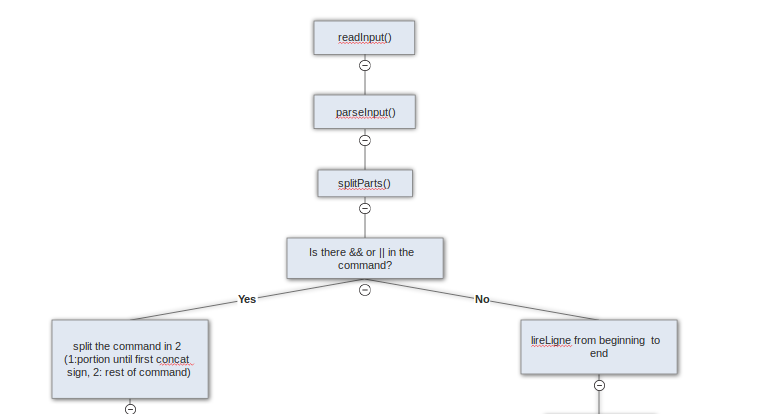
\includegraphics[width=\textwidth,height=\textheight,keepaspectratio]{codepartie1}
\\
\\
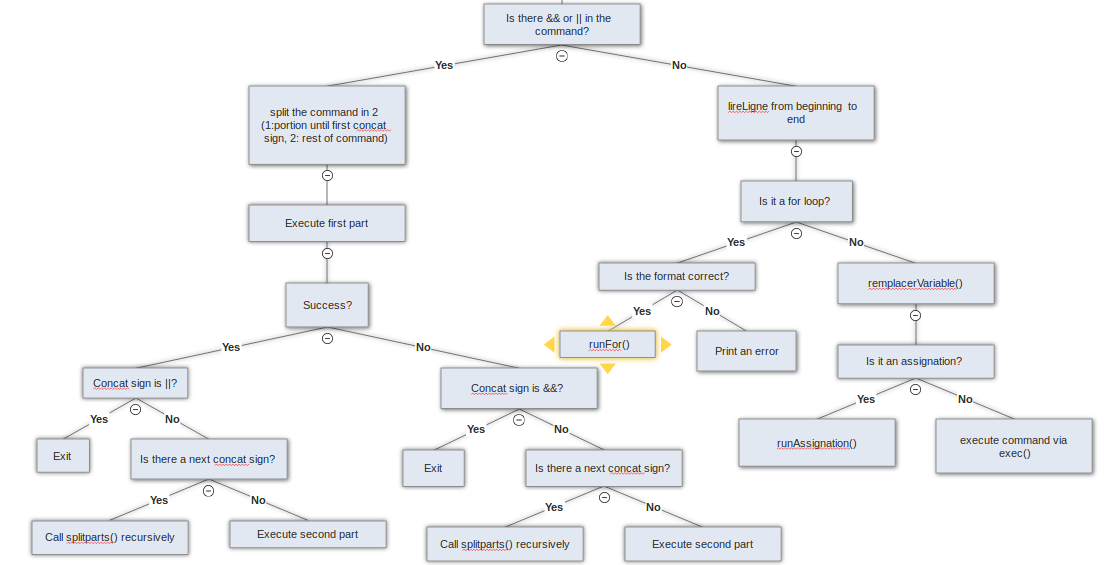
\includegraphics[width=\textwidth,height=\textheight,keepaspectratio]{codepartie2}


\section{Faiblesses et Améliorations possibles}

\begin{enumerate}
\item Couplage : même si ce cours n’en est pas un de génie logiciel, il est clair que notre code est structuré de façon à ce que beaucoup d’appels entre méthodes sont nécessaires. De plus, les méthodes ont presque toutes besoin de leur passer en argument le char**. Idéalement, nous voudrions dès le début splitter les informations et seulement envoyer celles dont chaque méthode a besoin via un pointeur. 
\item Orthographe : puisque nous faisons un parsing initial du input selon les espaces, notre terminal est très restrictif au niveau de la syntaxe. Certains espacements sont problématiques en bash donc c’est normal, mais d’autres devraient être acceptés (par exemple avec ou sans espace devant le “ ; “ ), mais nous avons développer selon le seul exemple de for qui nous était donné au départ. 

\item Algorithme : à plusieurs reprises dans le code, nous devons looper dans la commande pour chercher certains éléments (des “;”, des “:”, la bonne formulation du for, etc.). Cela n’est pas très optimal au niveau du temps d’exécution, car pour n lettres, on a une complexité de O(n) par recherche. Si l’usager rentre une grande commande, cela peut augmenter rapidement, mais il sera pratiquement impossible d'arriver à une meilleur borne O sans utiliser d'autres types de programmation ou sans utiliser de ressources supplémentaires.

\item Allocation de mémoire : L’outil valgrind nous a grandement aidé à réduire les allocations et à les frees, mais parfois nous ne pouvions free un élément dans le scope dans lequel il était déclaré sans affecté le résultat. Donc il y a des fuites mémoires qui se produisent. 
%reste a completer le dernier item

\end{enumerate}










%% ¡¡ REMPLIR ICI !!

\end{document} 